\chapter{Electronics Studies\label{chap:electronics}}
For a heavy MIP $\dv{E}{x} \approx \SI{2.1}{\mega\electronvolt\per\centi\metre}$, a \lartpc\ has a charge yield of $\order{\SI{1}{\femto\coulomb\per\milli\metre}}$ as explained in Chapter~\ref{chap:lartpc}.
The readout electronics need to be able to reliably digitise this charge.
This chapter aims to outline the challenges based on present designs and then present several tests of future approaches addressing them.

\section{Existing Chain\label{sec:electronics_existing}}
Contemporary electronics schemes shall be introduced by looking at the existing readout chain at LHEP at the University of Bern.
It was originally designed for the \AT\ experiment and a more detailed description can be found in~\cite{AT_larasic}.

The charge collected by the readout plane is amplified by LARASIC4*~\cite{larasic} cryogenic charge amplifiers developed by Brookhaven National Laboratory (BNL) for MicroBooNE~\cite{uboone}.
A performance characterisation of these application-specific integrated circuits (ASICs) can be found in~\cite{AT_larasic}.
Their main features include

\begin{itemize}
	\item \num{16} channels per ASIC;
	\item low noise charge amplifiers incorporating high-order filters;
	\item per channel programmable gain of \SIlist[list-final-separator = { or }]{4.7; 7.8; 14; 25}{\milli\volt\per\femto\coulomb};
	\item per channel programmable filter peaking time of \SIlist[list-final-separator = { or }]{0.5; 1.0; 2.0; 3.0}{\micro\second};
	\item built-in test capacitance connected to dedicated external test pulse input for calibration;
	\item and a power dissipation \SI{< 10}{\milli\watt} per channel.
\end{itemize}

\begin{figure}[htb] %TODO: change ASIC picture
	\centering
	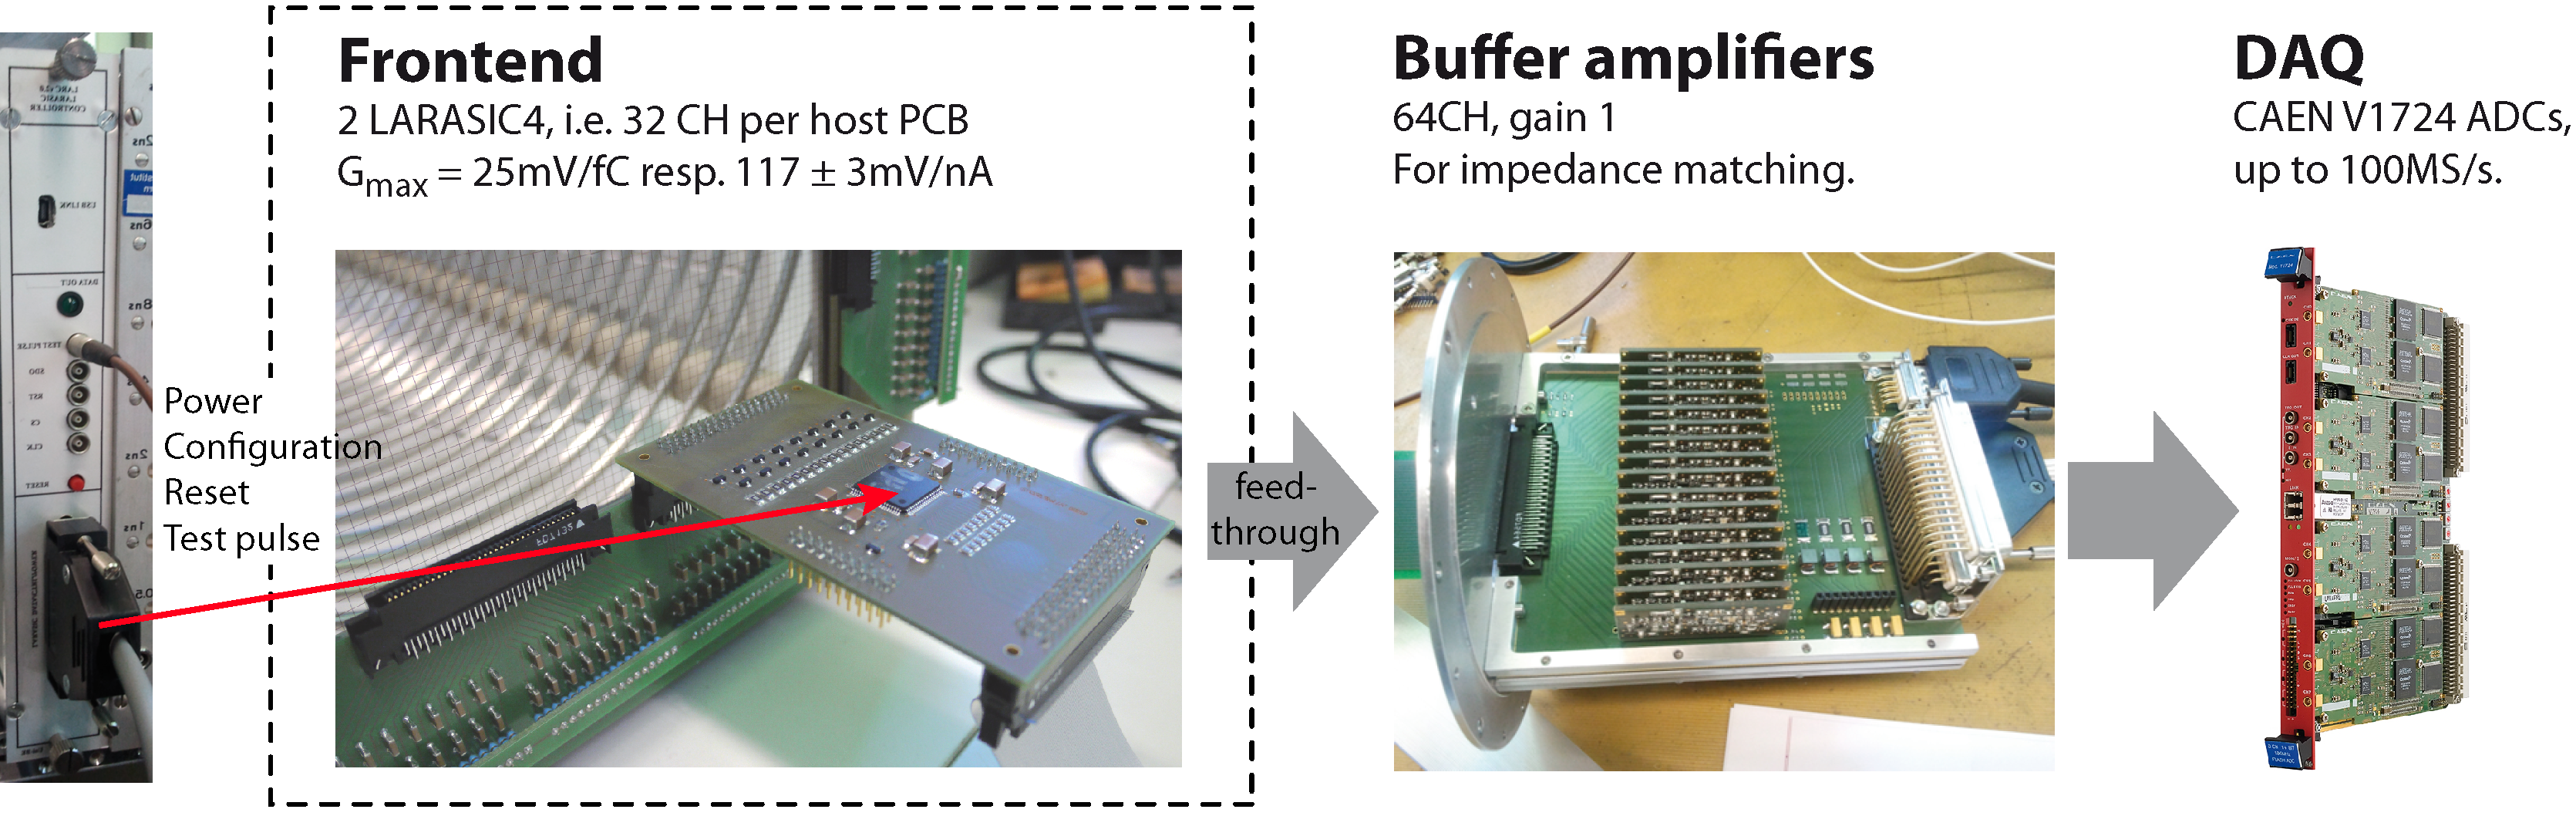
\includegraphics[width=\textwidth]{viper/ReadoutChain_old}
	\caption{Readout chain used for the pixel test. The picture of the LARASIC cryogenic front-end preamplifiers shows them installed in an older wire readout setup.~\cite{AT_larasic}}
	\label{fig:viper_readoutChain_old}
\end{figure}

The cryogenic preamplifiers are mounted as close as possible to the readout in order to minimise noise pick-up on these very sensitive lines.
Via an inter-integrated circuit (I$^2$C) bus, LARASICs can be programmed to the different aforementioned configurations.
For this purpose, they are connected to a bespoke NIM module housing an Arduino which generates the I$^2$C signals, a test pulse generator, and multiple low-noise voltage regulators providing power to the LARASICs.
The output of the preamplifiers is fed to buffer amplifiers mounted on top of the signal feedthrough by means of flexible Kapton ribbon cables.
The buffers operate at room temperature, have a unity gain, and match the output impedance of the LARASICs to the \SI{50}{\ohm} input impedance of the downstream digitisers.
From the buffers, the signals are routed via \SI{50}{\ohm} unbalanced coaxial lines to \emph{CAEN V1724}\footnote{\url{http://www.caen.it}} \SI{14}{bit} digitisers mounted in a VME crate.
For debugging purposes, the output of the buffers can be routed to an oscilloscope via a coaxial T-piece.
Finally, the digital data is read out from the VME crate via a fibre-optic link by a standard PC.
Figure~\ref{fig:viper_readoutChain_old} depicts the entire readout chain.
The complete analogue signal path from the pixel plane to the VME digitisers is single-ended and thus prone to ground loops and all associated noise problems.

\begin{figure}[htb] %TODO: picture
	\centering
	
\includegraphics[width=\textwidth]{placeholder}
	\caption{Event from the first measurement campaign of the pixel prototype.}
	\label{fig:viper_noisy-event}
\end{figure}

During the first pixelated readout measurement campaign, it became apparent that the data was significantly impaired by noise.
As can be seen in Figure~\ref{fig:viper_noisy-event}, the noise amplitude is similar over multiple channels.
This implies a common mode component that cannot originate from inductive pick-up.
Instead, the noise is likely generated by self-oscillating parts of the signal path due to ground loops and parasitic impedances.
For the second measurement campaign, different steps were take to mitigate this behaviour through modifications to detector location, power supply, signal path, and intrinsic capacitance.

A correlation between noise levels and the running state of the air condition in the utility room next to the lab was found.
Therefore, the experimental setup was moved away from the wall facing the utility room.

A decoupled clean power grid was built in the lab.
A Motor Generator (M-G set) separates the lab grid mechanically from the building power supply.
Thus, any noise present on the latter is prevented from entering the experimental setup.
Furthermore, this decouples the lab grid entirely from the building ground preventing ground loops via electric mains.

The signal path from the impedance-matching buffer amplifiers to the digitisers---i.e. the warm signal path---was changed from single-ended to differential signalling.
For conventional single-ended signalling, the signal is measured as the voltage or current difference between a signal conductor and a ground common to the signal source and the signal sink.
Using a common ground as signal return path can have several undesired effects.
To shield the signal conductor, it is usually enclosed in a ground shield.
If the latter is connected on both sides, a ground loop can result for instance in combination with a shared power supply ground.
Ground loops can pick up noise through induction if the resistance along the loop is high enough.
A second way to couple noise into a single-ended system is by shifting the potential on the common ground away from the reference voltage or current, for instance due to high currents flowing through a lossy ground connection.
Because the signal is always measured against the common ground, it will be distorted.
In differential signalling, the signal is not measured between a signal conductor and ground but instead between two signal conductors.
This works by putting an inverted waveform of the signal on a second conductor.
The signal is recovered by taking the difference between to two signal conductors.
As a result, the signal sink needs not be connected to the same ground as the signal source because the signal is independent of ground.
Ground loops can thus be avoided in the signal path.
Furthermore, the effects of noise pick-up on the signal lines is drastically reduced.
Due to the completely symmetric signal path, inductive noie pick-up is equal on both signal conductors as opposed to single-ended signals where the signal path is not symmetric.
In the signal sink, the difference between the two symmetric signal conductors is formed and everything that is present on both of them, such as the inductively picked up noise, cancels out.
In the pixel prototype setup, differential signalling was realised by replacing the buffer amplifiers by single-ended to differential amplifiers and inserting another stage upstream of the digitisers to change the signal back to \SI{50}{\ohm} single-ended, matching the input of the digitisers.
Like this, noise pick-up outside the cryostat could be reduced as well as sensitivity to ground loops between the detector and the DAQ rack.

A source of noise was identified in the layout of the pixel readout plane.
It was found that due to several ground planes and long tracks in the PCB, parasitic capacitances were very high, in particular for pixel channels.
This is problematic because for high enough frequencies---determined by $RC$---, the input is shorted to ground creating a ground loop again.
Through this capacitive coupling to ground, the system can start to oscillate.
One evidence for this is that the noise is equal over multiple channels, so-called common-mode noise.
More specifically, the noise is equal over groups of channels.
Investigating this, it was found that these groups correspond to channels of roughly equal parasitic capacitance.
Also, the noise amplitude is higher on channels with higher capacitance.
To solve this problem, the PCB design was optimised by removing unnecessary ground planes, routing signal tracks outside necessary ground planes and increasing the thickness of the PCB.

\begin{figure}[htb] %TODO: picture
	\centering
	
\includegraphics[width=\textwidth]{placeholder}
	\caption{Event from the second measurement campaign of the pixel prototype after improving the readout chain.}
	\label{fig:viper_good-event}
\end{figure}

As can be seen from Figures~\ref{fig:viper_noisy-event} and~\ref{fig:viper_good-event}, there is a significant decrease in noise after commissioning all of the above improvements to the readout chain.
This can also be seen from Figures~\ref{fig:viper_snr-noisy} and~\ref{fig:viper_snr-good} depicting the signal to noise ratio of the two measurement campaigns.

\begin{figure}[htb] %TODO: picture
	\centering
	
\includegraphics[width=\textwidth]{placeholder}
	\caption{Signal vs noise using the old readout chain.}
	\label{fig:viper_snr-noisy}
\end{figure}

\begin{figure}[htb] %TODO: picture
	\centering
	
\includegraphics[width=\textwidth]{placeholder}
	\caption{Signal vs noise after imrpoving the readout chain.}
	\label{fig:viper_snr-good}
\end{figure}


\section{Improved Cold Electronics for Pixelated Readouts\label{sec:electronics_pixels}}